\chapter{Einleitung}

\section{Motivation}
Um im Unterricht Schülern und Studenten das Programmieren und Konstruieren von Robotern zu erläutern, ist Lego Mindstorms mit dem programmierbaren Baustein NXT eine gute Wahl. Das Ziel dieser Arbeit ist es das Programmieren von Lego Mindstorms Robotern zu vereinfachen und gleichzeitig die Grenzen, die duch den Baustein NXT gesetzt sind, aufzulösen. Wir wollen die Möglichkeiten der Programmierung des NXT eins zu eins mit dem Minicomputer Raspberry PI abbilden. Damit ist es uns möglich eine einfache Programmierschnittstelle anzubieten und zusätzlich die vielen Möglichkeiten des Raspberry PIs für Studenten und Schüler zugänglich zu machen. 

In der folgenden Arbeit werden wir den, vom Raspberry PI gesteuerten, Lego Mindstorms Roboter LegoPI nennen.

Wir sehen den Raspberry PI als ein dem NXT überlegenes Steuerungsmodul, da auf dem Raspberry ein vollständiges Ubuntu Betriebssystem läuft. Ubuntu ist eine kostenlose Linux Distribution. Eine Überlegung der Autoren ist auf dem Ubuntu einen Webserver laufen zu lassen und dem Roboter über diesen aus der Ferne zu steuern.
Weiterhin soll es in dieser Arbeit ermöglicht werden, weitere Sensoren an den Raspberry PI anschließen zu können. Zwar gibt es für Lego Mindstorms eine Liste von Sensoren, wie z.B einen Lichtsensor, Tastsensor und Ultraschallsensor. Dieses Set an Sensoren ist allerdings durch Lego Mindstorms eingeschränkt.

Das Bereitstellen eines programmierbaren Roboters für jeden Schüler kann schnell teuer werden. Wir sehen die Verwendung eines Raspberry PI auch deshalb als Vorteil, weil ein Raspberry B+ mit 39,90 Eur den NXT 9841 mit 148,99 Eur preislich schlägt. \footnote{Preisvergleich des Raspberry PI 2 B+ und NXT 9841 auf www.amazon.de}

In dieser Arbeit werden wir uns darauf beschränken, alle Sensoren des NXT Bausatzes mit dem Raspberry PI zu verbinden. Zusätzlich soll es möglich sein, Motoren über den Raspberry zu steuern. Um prüfen zu können, ob der Raspberry PI den NXT im Unterricht ersetzen kann, werden wir einen Parqour, der auch von Schülern der Hochschule Mannheim absolviert werden muss, mit dem LegoPI durchlaufen.

Diese Arbeit wird zunächst die nötigen Grundlagen erklären, um die Implementierung des LegoPIs zu verstehen. Danach wird die technische Implementierung im Detail erläutert. Abschließend wird die von uns entwickelte neue Python API vorgestellt, mit welcher Studenten und Schüler in Zukunft ihre eigenen Roboter programmieren können.

\chapter{Grundlagen}
\section{Raspberry PI}
\label{Grundlagen:RaspberryPI}
%\index{Auszeichnungen!im Text}

Raspberry PI ist ein günstiger Computer in Kreditkartengröße, der viele Schnittstellen bietet, wie z.B HDMI, USB, Audio, GPIOs und Ethernet.
Das auf dem Raspberry PI ein vollständiges Linux Betriebssystem läuft, macht ihn besonders beliebt. Dies führt dazu, dass vieles was auf einem Desktoprechner läuft, auch auf einem Raspberry PI ausführbar ist.

\begin{figure}[h]
  \centering
  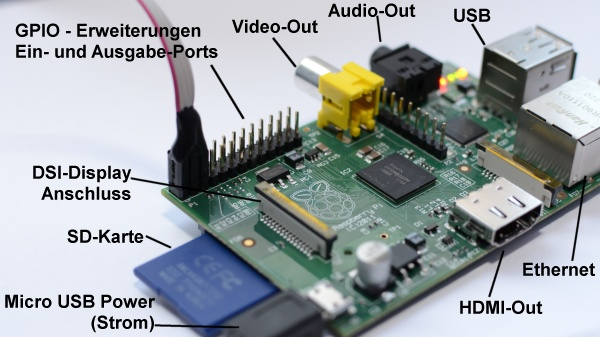
\includegraphics[width=15cm]{raspberrypi}
  \caption{Ein RaspberryPI 2 mit beschrifteten Schnittstellen. Quelle: http://www.portunity.de/blog/2013/februar/raspberry-pi-warum-ist-der-mini-computer-bei-unseren-mitarbeitern-so-beliebt.html}
  \label{Kap1:RaspberryPI}
\end{figure}

\section{NXT}
\label{Grundlagen:NXT}
%\index{Auszeichnungen!im Text}

Lego Mindstorms NXT ist ein Steuerungscomputer der Produktserie Lego Mindstorms. Der NXT hat ebenso wie der Raspberry PI Anschlüsse für USB- und Bluetooth Schnittstellen. Im Gegensatz zu Raspberry PI bietet der NXT schon von voreingebaute Anschlüsse für Sensoren und Motoren. 

\begin{figure}[h]
  \centering
  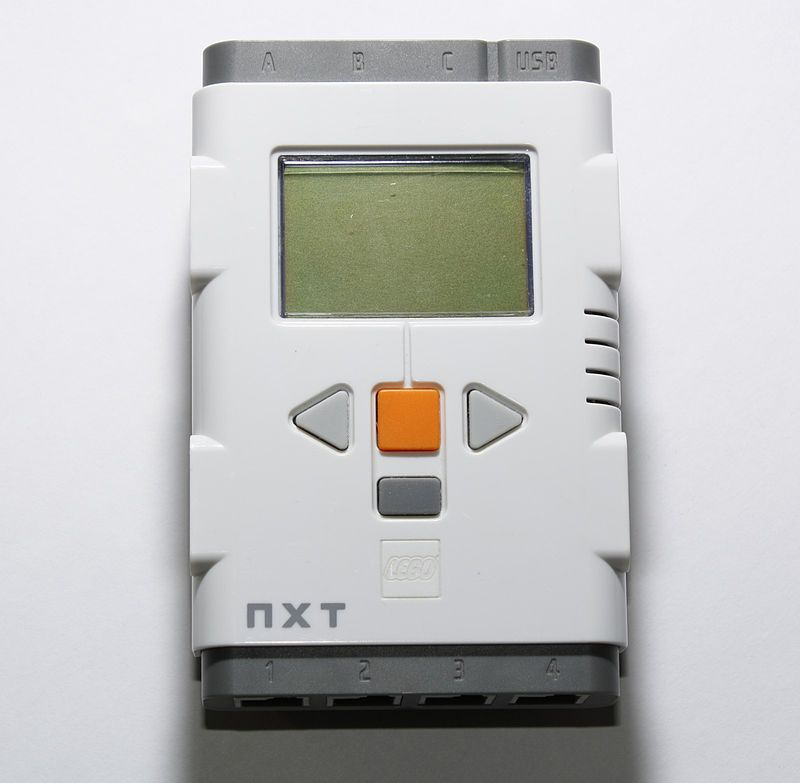
\includegraphics[width=12cm]{nxt}
  \caption{Ein NXT Baustein mit Anschlüssen für Motoren und Sensoren. Quelle: https://de.wikipedia.org/wiki/Lego-Mindstorms-NXT}
  \label{Kap1:NXT}
\end{figure}

\section{A/D-Wandler}

Ein Analog-Digital-Umsetzer, kurz A/D-Wandler, ist ein elektronisches Baustein, bei dem ein zeit-kontinierliches Eingangssignal in einzelne diskrete Werte abgetastet werden.

\section{Bussysteme}
In der Computerarchitekture ist ein Bus ein System, das Daten zwischen einzelnen Computerbestandteile überträgt.

\subsection{SPI}

Der Serial Peripheral Interface (SPI) Bus ist eine von Motorola entwickelte,  synchrone, serielle Kommunikationsschnittstelle, welche für die Übertragung von Daten über kurze Distanzen entworfen ist.  Häufige Anwendung findet der SPI in Embedded Systems. 

In Abbildung 2.3 ist der Aufbau von einem SPI Bus dargestellt.
Eine Kommunikation über SPI erfolgt über einen SPI Master und einen SPI Slave. Der SPI Master startet eine Kommunikation in dem er die SS Verbindung auf 0 Volt zieht und ein clock signal mit einer bestimmten clock frequency aktiviert. Die zu sendenden Signale werden dann, in der Frequenz die von SCLK vorgeben ist, über den MOSI (Master Out Slave In) übertragen. Der SPI ist ein single-master Protokoll, da lediglich ein Master die Kommunikation über alle Slaves steuert.

\begin{figure}[h]
  \centering
  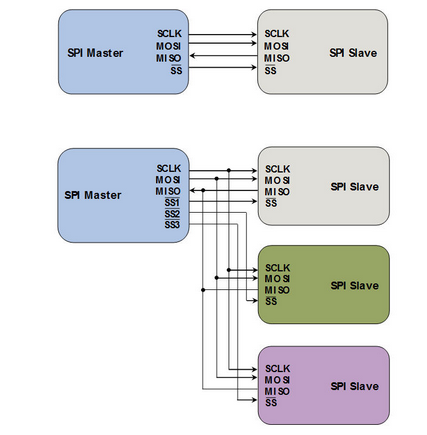
\includegraphics[width=12cm]{spi.png}
  \caption{SPI Kommunikation erfolgt über einen Puls der von SCLK gegeben ist und den Master und Slave synchronisiert. Über MOSI (Master IN Slave OUT) sendet der Master Signale an den Slave. Quelle: http://www.byteparadigm.com/applications/introduction-to-i2c-and-spi-protocols}
  \label{Kap1:SPI}
\end{figure}

\subsection{I2C}

I2C ist ein multi-master Protokoll mit zwei Datenleitungen. Über Serial Data (SDA) werden die Daten übertragen. Der SCL (Serial Clock) gibt die Frequenz der Datenübertragung an und synchronisiert somit die Kommunikationspartner. Jedes Gerät, welches an den Bus angeschlossen ist, bekommt eine 7 -bit slave address. Es können beliebig viele Geräte an den I2C angeschlossen werden. Die Daten werden in 8-bit Paketen übertragen. Die Datenraten können 100 kbps, 400 kbps oder 3.4 Mbps betragen. Diese verschiedenen Übertragungsraten werden auch standard mode, fast mode und high speed mode genannt.

Physikalisch besteht der I2C Bus aus zwei Leitungen und einer Ground Leitung (siehe Abbildung 2.4). Die aktiven Leitungen sind bi-direktional. Im I2C Standard ist definiert, dass jedes I2C Gerät welches Daten übersenden will, die Rolle eines Masters annimmt und alle anderen Geräte in diesem Moment Slaves sind.

\begin{figure}[h]
  \centering
  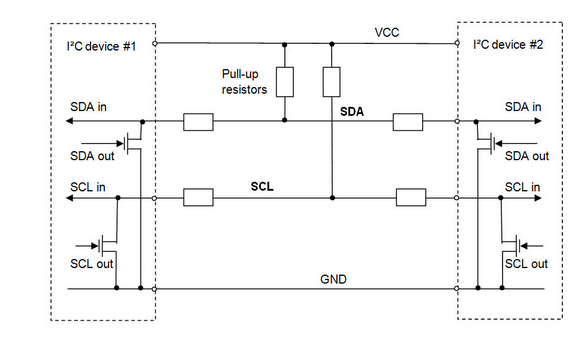
\includegraphics[width=15cm]{i2c}
  \caption{Zwei I2C Geräte sind über SDA und SCL verbunden. Diese beiden Leitungen sind über pull-up Widerständen mit VCC verbunden. Quelle: http://www.byteparadigm.com/applications/introduction-to-i2c-and-spi-protocols/}
  \label{Kap1:I2C}
\end{figure}

\clearpage

\subsection{Sensoren}
Unter Sensoren versteht man Komponenten, in denen eine physikalische oder chemische Veränderung in ein geeignetes Nutzsignal erfasst oder gemessen wird.

Im folgenden werden die Sensoren beschrieben, die in dieser Arbeit in Betrieb genommen werden.

\subsubsection{NXT Lightsensor}
Der NXT Lichtsensor misst, wie viel Licht  in den Sensor fällt. Dies geschieht über einen light-dependent resistor (LDR), der ein variabler Widerstand ist und niedriger wird, je mehr Licht hereinfällt. Der Lichtsensor verfügt ebenfalls über eine externe Lichtquelle. Mit dieser ist es möglich, auch in dunklen Lichtverhältnissen zwischen Oberflächen zu unterscheiden.

\begin{figure}[h]
  \centering
  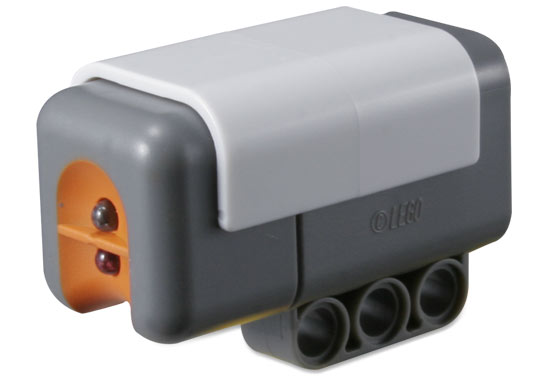
\includegraphics[width=4cm]{lightsensor}
  \caption{NXT Lightsensor mit dem LDR oben und einer externen Lichtquelle unten.}
  \label{Kap1:Lightsensor}
\end{figure}

\subsection{Tastsensor}

Der Tastsensor ist ein einfacher Sensor, der die Werte 1 für gedrückt und 0 für nicht gedrückt darstellen kann. In dieser Arbeit wird dieser Sensor unter anderem dazu verwendet, den Roboter zu starten. Ist der Schalter gedrückt, wird ein Startskript ausgeführt.

\begin{figure}[h]
  \centering
  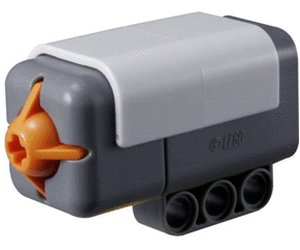
\includegraphics[width=4cm]{tast}
  \caption{NXT Tastsensor}
  \label{Kap1:tast}
\end{figure}

\section{GPIO}
Ein General Purpose Input/Output (GPIO) ist eine einfache digitale Schnittstelle mit der eine Folge von Einsen und Nullen übertragen werden können.
Der Raspberry PI 2 bietet 40 GPIOs, welche jeweils als Eingabe oder Ausgabe Pins geschaltet werden können.

\chapter{Technische Implementierung}

\section{Elektronische Bauteile}

\subsection{Motor}\label{eb:motor}

% Tabelle
\begin{table}[!ht]
\centering
\rmfamily
\caption{Pinbelegung Motor}
\renewcommand{\arraystretch}{1.1}
\sffamily
\begin{footnotesize}
\begin{tabular}{r | l l}
\toprule
\textbf{Pin} & \textbf{Farbe}  & \textbf{Belegung}\\
\midrule
1 & Weiß & Motor +9V; PWM-Steuerung \\
2 & Schwarz & Motor -9V; PWM-Steuerung \\
3 & Rot & Ground \\
4 & Grün & +4,3V Versorgungsspannung \\
5 & Gelb & Motorencoder (Quadratur-Encoder, Kanal a) \\
6 & Blau & Motorencoder (Quadratur-Encoder, Kanal b) \\
\bottomrule
\end{tabular}
\end{footnotesize}
\label{eb:motor:tbl}
\end{table}

Die Steuerung des Motors erfogt über eine 9V Spannung. Für die Regulierung der Geschwindigkeit wird eine Pulsweitenmodulation verwendet. Die max. Stromstärke liegt bei 700mA für den Motor.  Die Versorgungsspannung an Pin 4 versorgt den Rotationssensor mit Strom. Mittels des Rotationssensors kann die genaue Rotationsposition des Motors bestimmt werden. Dieser Sensor kann über die Pin's 5 und 6 ausgelesen werden. Der Rotationssensor, des Motors wurde in diesem Projekt nicht weiter behandelt.


\subsection{Sensoren}\label{eb:sensor}

Im folgenden werden die Sensoren des NXT näher beschrieben. Für jeden Sensor wird außerdem die Pinbelegung aufgelistet und der Strombedarf.

\subsubsection{Tastsensor}
% Tabelle
\begin{table}[!ht]
\centering
\rmfamily
\caption{Pinbelegung Tastsensor}
\renewcommand{\arraystretch}{1.1}
\sffamily
\begin{footnotesize}
\begin{tabular}{r | l l}
\toprule
\textbf{Pin} & \textbf{Farbe}  & \textbf{Belegung}\\
\midrule
1 & Weiß & Trigger \\
2 & Schwarz & - \\
3 & Rot & Ground \\
4 & Grün & - \\
5 & Gelb & - \\
6 & Blau & - \\
\bottomrule
\end{tabular}
\end{footnotesize}
\label{tastsensor:tbl}
\end{table}
Der Tastsensor gehört zu den analog Sensorn vom NXT. Im Normalzustand ist der Tastsensor geöffnet (no: Normal Open). Die Leistungsaufnahme des Tastsensors ist im geöffneten zustand mit 2,2mA sehr gering. Im geschlossenen Zustand liegt die Stromaufnahme bei 0mA.


\subsubsection{Tonsensor}
% Tabelle
\begin{table}[!ht]
\centering
\rmfamily
\caption{Pinbelegung Tonsensor}
\renewcommand{\arraystretch}{1.1}
\sffamily
\begin{footnotesize}
\begin{tabular}{r | l l}
\toprule
\textbf{Pin} & \textbf{Farbe}  & \textbf{Belegung}\\
\midrule
1 & Weiß & Analoges Tonsignal \\
2 & Schwarz & Ground \\
3 & Rot & Ground \\
4 & Grün & +4,3V Versorgungsspannung \\
5 & Gelb & Moduswahl dB/dBA \\
6 & Blau & Direkter Ausgang \\
\bottomrule
\end{tabular}
\end{footnotesize}
\label{tonsensor:tbl}
\end{table}
Der Tonsensor war nicht Teil dieses Projektes, jedoch wird er zur Vollständigkeit hier aufgeführt. Auch der Tonsensor ist ein Analogsensor. Dieser Senesor misst den Schalldruck zwischen 55 dB und 90 dB. Bei der Decibelskala ist zu beachten, dass es sich hier um eine logarithmische Skalierung handelt. Somit nimmt der Mensch eine Erhöhung der Lautstärke um 10 dB als Verdopplung der Lautstärke wahr. Die Stromaufnahme des Tonsensors liegt bei 2,0mA.

\subsubsection{Lichtsensor}
% Tabelle
\begin{table}[!ht]
\centering
\rmfamily
\caption{Pinbelegung Lichtsensor}
\renewcommand{\arraystretch}{1.1}
\sffamily
\begin{footnotesize}
\begin{tabular}{r | l l}
\toprule
\textbf{Pin} & \textbf{Farbe}  & \textbf{Belegung}\\
\midrule
1 & Weiß & Analoges Lichtsignal \\
2 & Schwarz & Ground \\
3 & Rot & Ground \\
4 & Grün & +4,3V Versorgungsspannung \\
5 & Gelb & Lichtquelle Ein/Aus \\
6 & Blau & - \\
\bottomrule
\end{tabular}
\end{footnotesize}
\label{lichtsensor:tbl}
\end{table}

Der Lichtsensor ist auch ein analoger Sensor. Über einen lichtempfindlichen Widerstand (LDR) kann dieser Sensor die Helligkeit messen. Der Sensor hat zwei Modis. Der erste Modus ist \emph{Umgebungslicht Modus} mit einer Stromverbrauch von 2,5mA.  Im \emph{Reflektions Modus} wird eine kleine LED aktiviert und der Stromverbrauch steigt so auf 15 mA.

\subsubsection{Ultraschallsensor}
% Tabelle
\begin{table}[!ht]
\centering
\rmfamily
\caption{Pinbelegung Ultraschallsensor}
\renewcommand{\arraystretch}{1.1}
\sffamily
\begin{footnotesize}
\begin{tabular}{r | l l}
\toprule
\textbf{Pin} & \textbf{Farbe}  & \textbf{Belegung}\\
\midrule
1 & Weiß & +9V Versorgungsspannung \\
2 & Schwarz & Ground \\
3 & Rot & Ground \\
4 & Grün & +4,3V Versorgungsspannung \\
5 & Gelb & I2C-Kommunikation SCL (Serial Clock) \\
6 & Blau & I2C-Kommunikation SDA (Serial Data) \\
\bottomrule
\end{tabular}
\end{footnotesize}
\label{eb:ultraschall:tbl}
\end{table}

Der ultraschall Sensor ist ein digitaler Sensor. Das bedeutet, dass das Signal mittels I2C-Bus übertragen wird. Mit diesem Sensor können Distanzen zwischen  0cm und 255cm gemessen werden. Es ist der einzigste Sensor der zusätzlich zu der normalen Versorgungsspannung von 4,3V noch eine 9V Versorgungsspannung benötigt.

\subsection{SN754410}\label{eb:pwm}
%Figure
\begin{wrapfigure}{r}{0.65\textwidth}
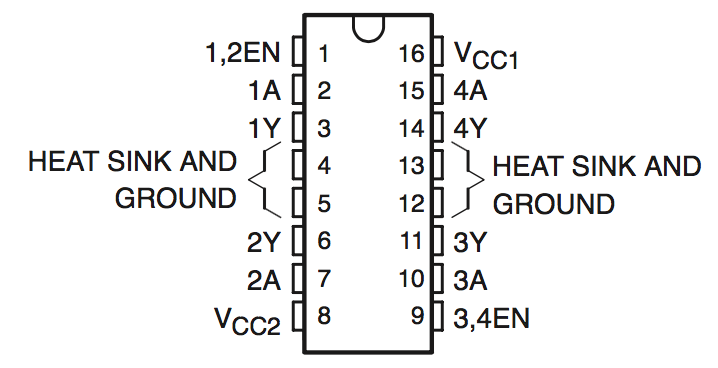
\includegraphics[width=0.9\linewidth]{bauelemente/sn754410}
\caption{SN754410}
\label{eb:fig:sn754410}
\end{wrapfigure}
Der SN754410 ermöglicht das Steuern der zwei Motoren mit einer max Stromstärke von 1A (max Stromaufnahme eines Motors 700 mA) bei 9V. Die von uns  geschriebene Software steuert den Chip so an, dass über eine Pulsweitenmodulation die Geschwindigkeit des Motors beliebig angepasst werden kann. Durch die Pulsweitenmodulation ist die Wärmeentwicklung sehr gering. Daher ist eine Kühlung dieses Bauteils nicht notwendig.

Über jeweils zwei GPIO-Pins kann so ein Motor gesteuert werden.

\subsection{MCP3008}\label{eb:adwandler}
%Figure
\begin{wrapfigure}{r}{0.4\textwidth}
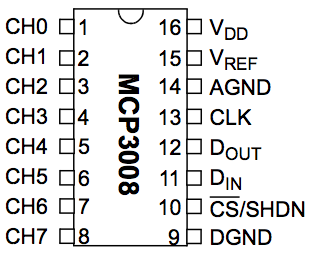
\includegraphics[width=0.9\linewidth]{bauelemente/mcp3008}
\caption{MCP3008}
\label{eb:mcp3008}
\end{wrapfigure}
Der MCP3008 ist ein Analog/Digital-Wandler (A/D-Wandler). Dieses Bauteil wird über den SPI-Bus am Raspberry Pi angeschlossen. Über den 8 Eingänge (CH0-CH7) lassen sich 8 verschiedene analoge Sensore anschließen. Der A/D-Wandler macht aus dem analogen Einganssignal einen Bitstream, der über den SPI-Bus übertragen wird.

Über vier GPIO-Pins können so 8 analoge Sensoren gesteuert werden.

\section{Elektronischer Aufbau}

\subsection{Motor}
%Figure
\begin{wrapfigure}{r}{0.65\textwidth}
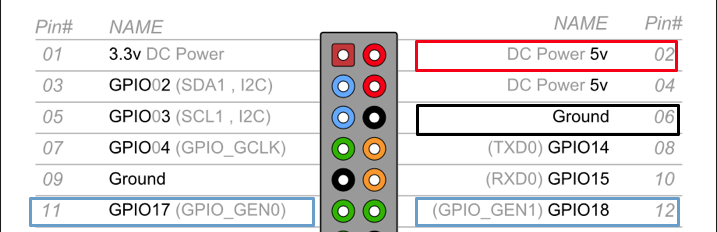
\includegraphics[width=0.9\linewidth]{schaltung/motor-pin}
\caption{GPIO Belegung Motor}
\label{ea:motor-pin}
\end{wrapfigure}
An der Pinbelegung des Motors \ref{eb:motor:tbl} ist zu erkennen, dass der Motor eine Spannung von 9V benöigt. Die Versorgungspanng von 4,3V ist für den eingebauten Controller im Motor. Pin 1 und 2 des Motors müssen mit dem in \ref{eb:pwm} beschriebenen Bauteil verbunden werden (hier Pin 14 und 10 von 754410). Die 9V Motorspannung liegt an Pin 8 (SN754410) an und kommt von einem zusätzlich 9V-Block. Über die Pins 15 und 11 wird das Bauteil an 2 GPIO's angeschlossen. Weitere benötigte Verbindungen sind die GND, welche alle zusammen verbunden werden und die Versorgungspannung von 4,3V-5V.

Eine Vollständige Belegung der Pins für den Probeaufbau befindet sich in Abbildung \ref{ea:motor-pin}

%Figure
\begin{figure}[h]
  \centering
  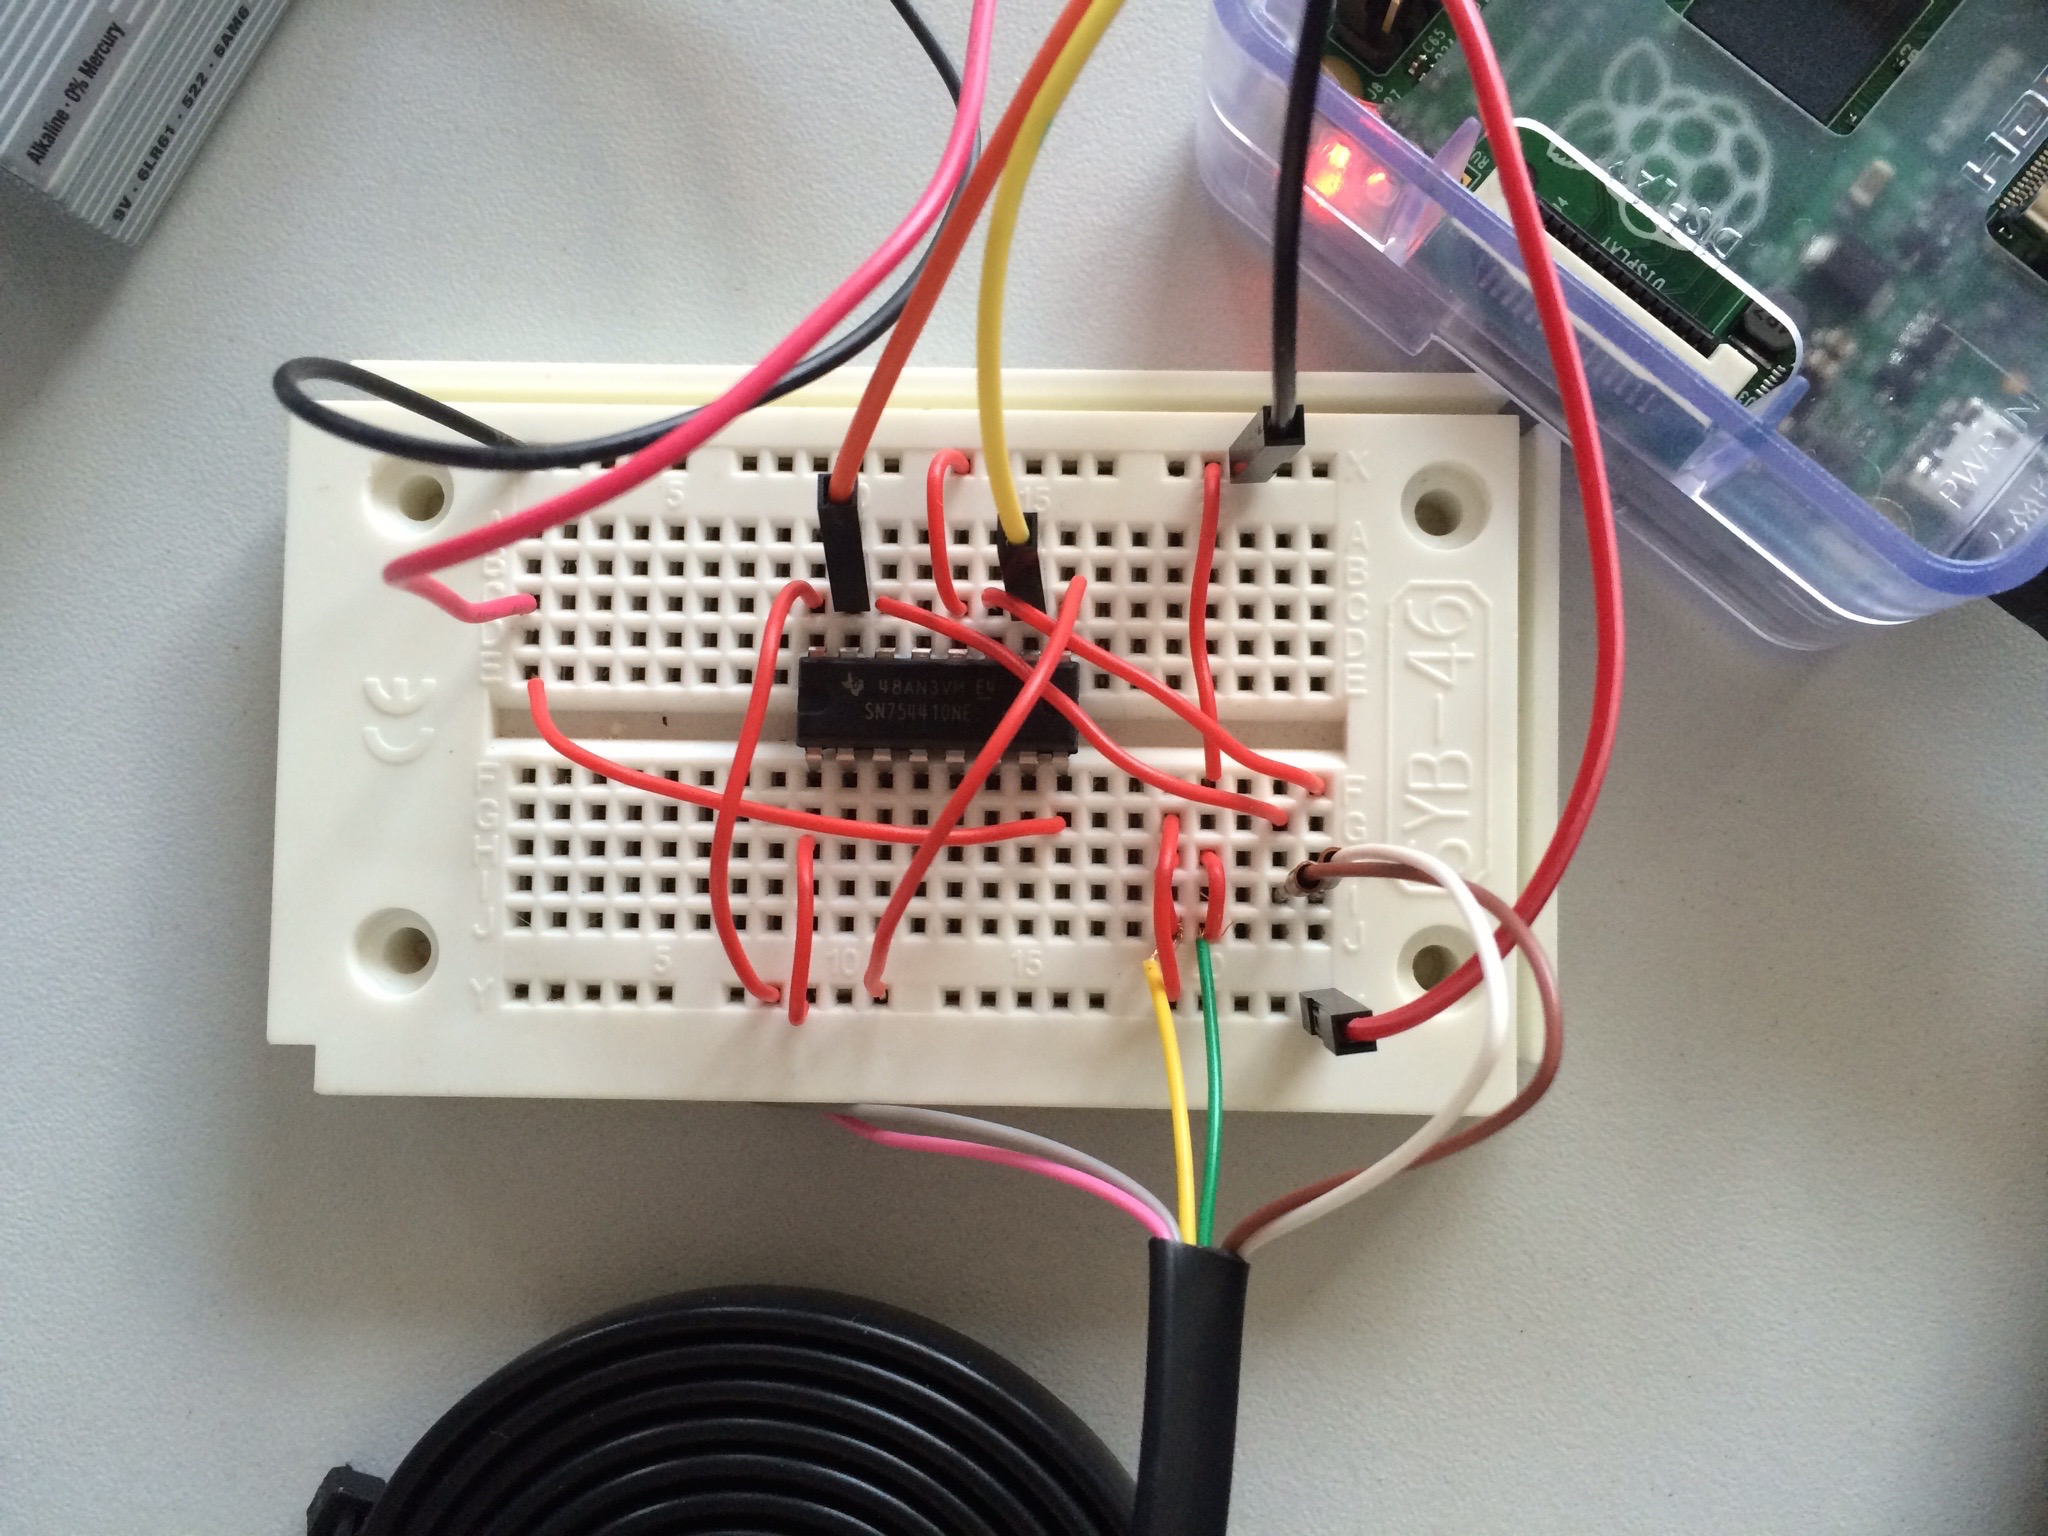
\includegraphics[width=12cm]{schaltung/motor}
  \caption{Probeaufbau Motor}
  \label{schaltung:motor}
\end{figure}

\subsection{Sensor}
%Figure
\begin{wrapfigure}{r}{0.65\textwidth}
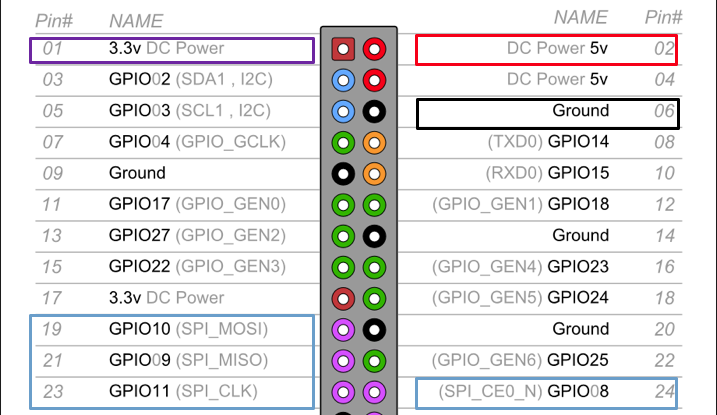
\includegraphics[width=0.9\linewidth]{schaltung/sensor-pin}
\caption{GPIO Belegung Sensor}
\label{ea:sensor-pin}
\end{wrapfigure}

Die Versorgungspannung für den MCP3008 ist hier 3,3V und die Versorgungspannung für die Sensoren sind 4,3V-5V vom Raspberry Pi. Die analogen Sensoren werden an CH0-CH7 des A/D-Wandlers über eine Spannungsteilerschaltung angeschlossen. Der Spannungteiler wird mit einem 10 kOhm Widerstand realisiert (in der Probeschaltung 2* 4,7kOhm in Reihe). Mit vier Anschlusskabeln wird der A/D-Wandler über den SPI-Bus am Raspberry Pi angeschlossen. Die Erdung geschieht auch über den Raspberry. Bei dem Spezialfall \emph{Lichtsensor} wird zusätzlich für die Lichtquelle eine Versorgungsspannung benötigt. Da der PIN 5 bei dem \emph{Tastsensor} nicht belegt ist, wird standartmäßig überall der Pin 5 an 4,3V-5V angeschlossen.

%Figure
\begin{figure}[h]
  \centering
  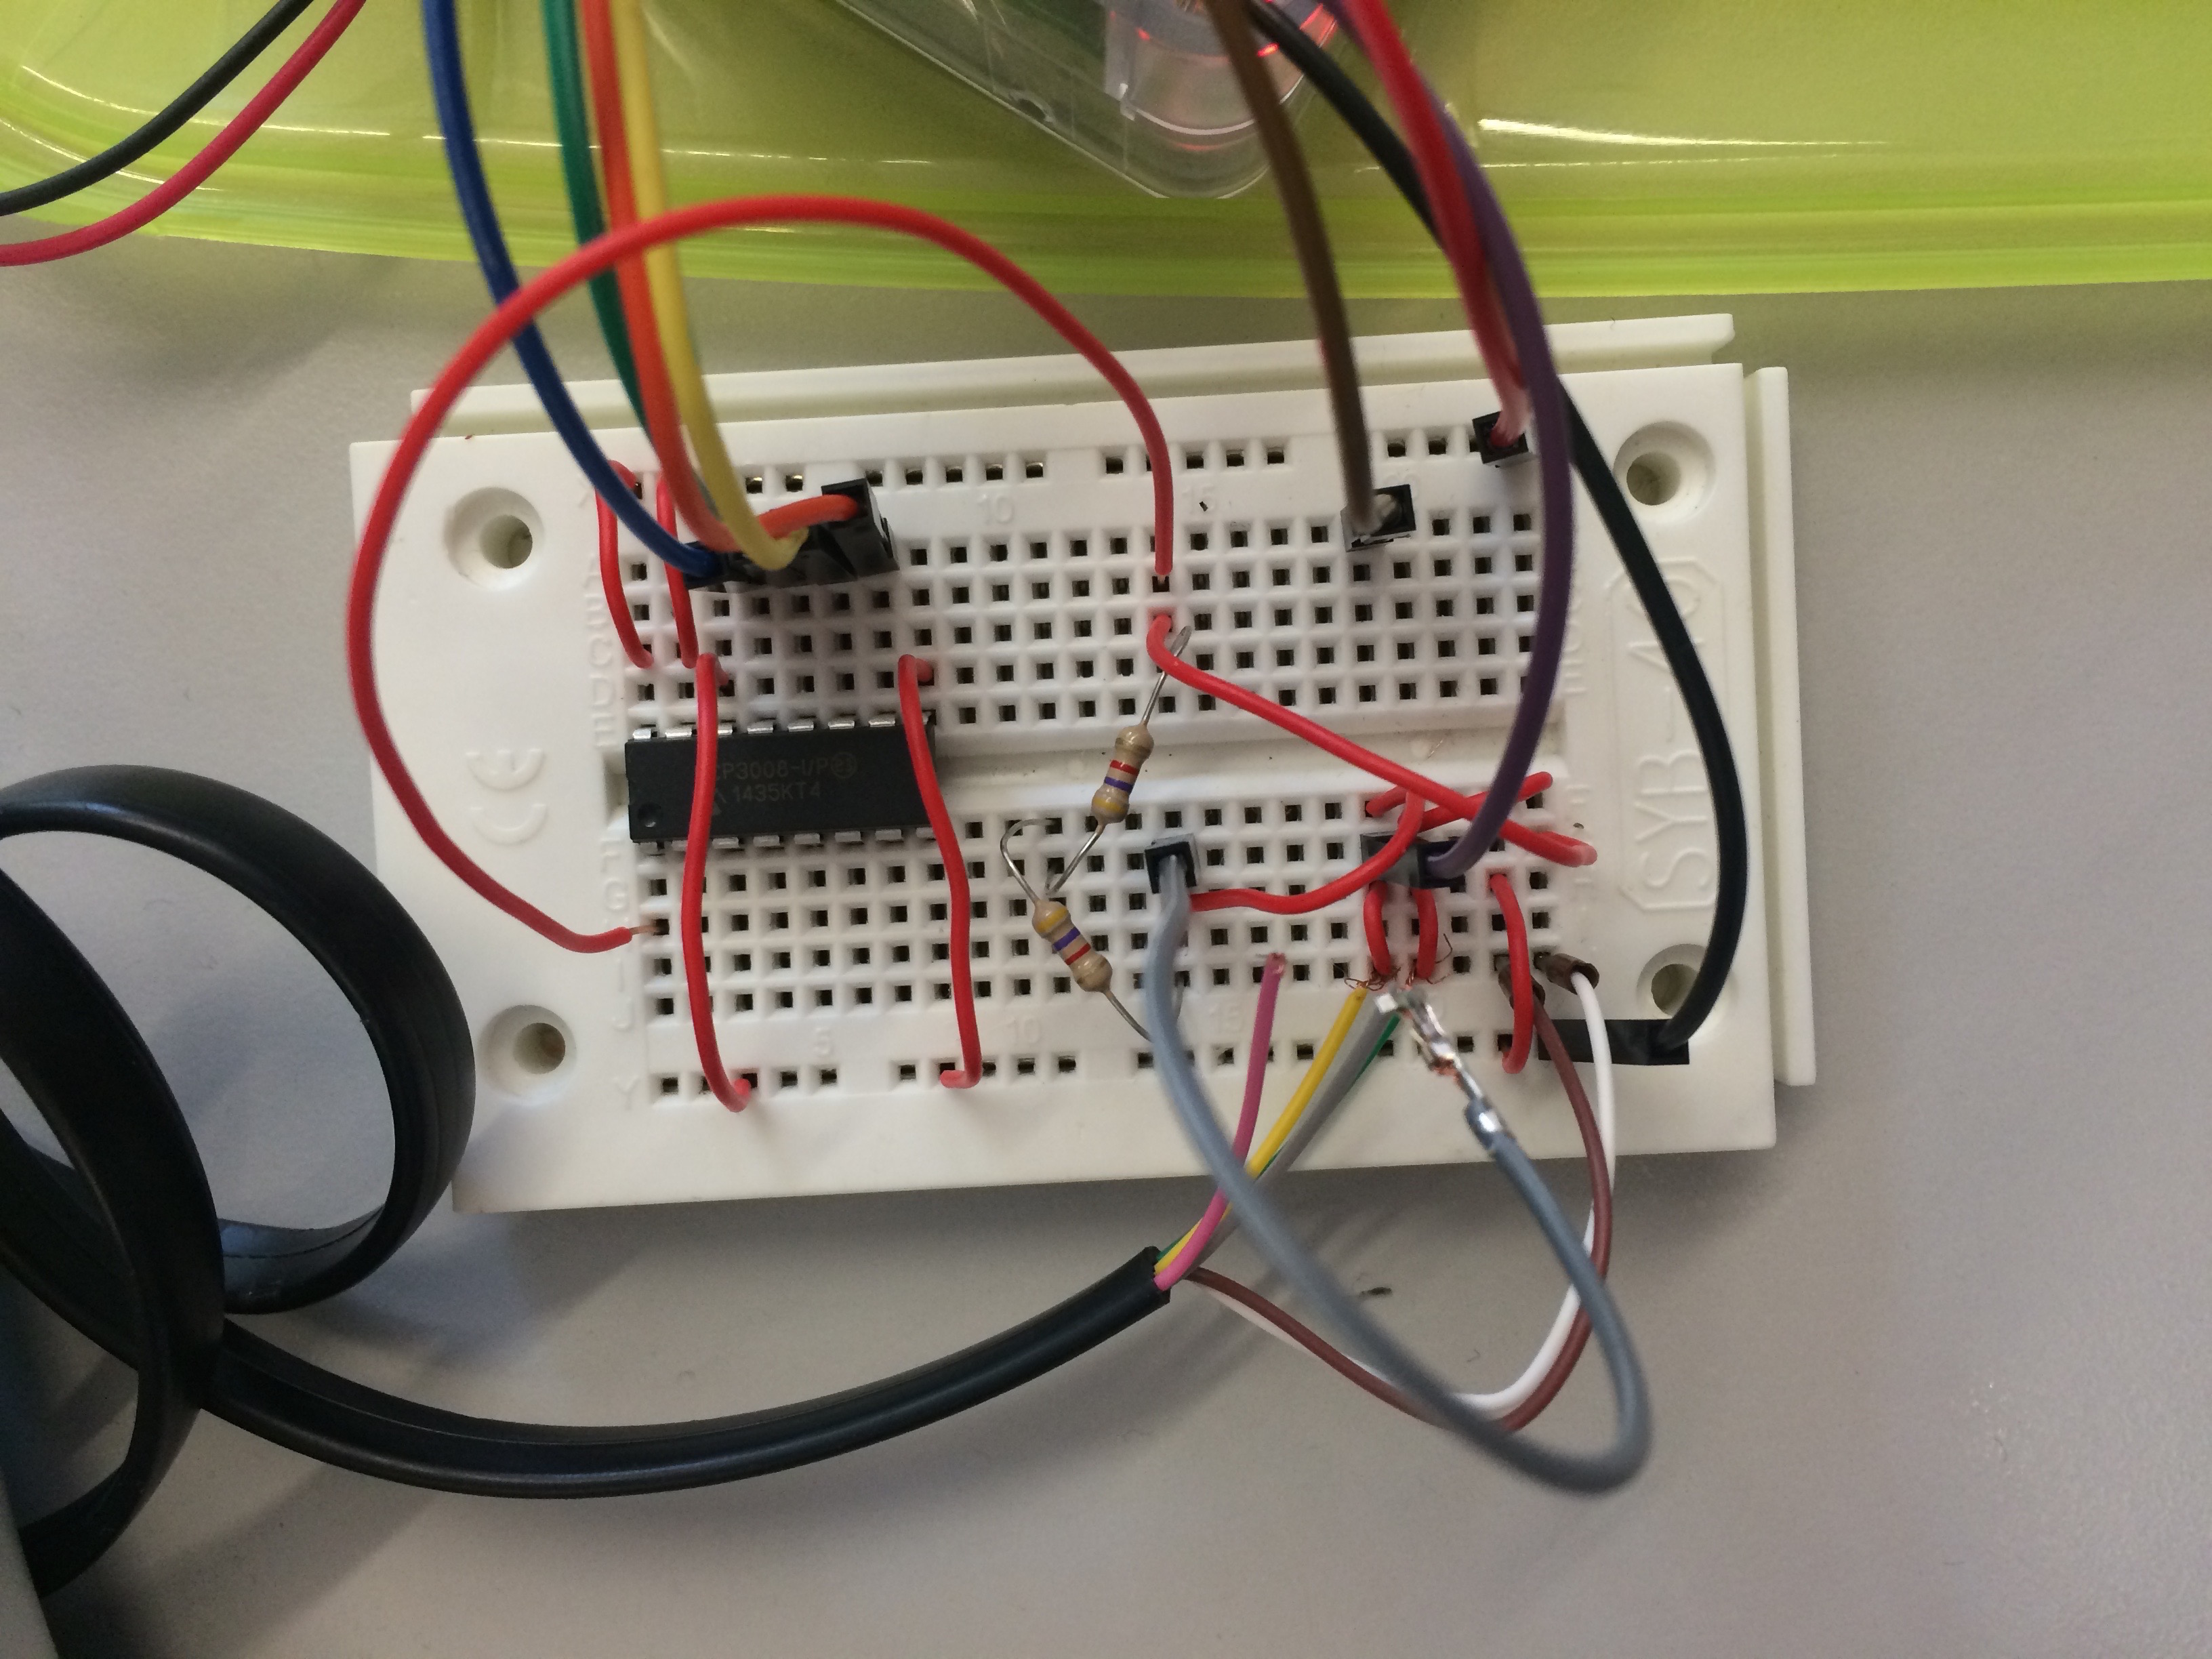
\includegraphics[width=12cm]{schaltung/sensor}
  \caption{Probeaufbau Sensor}
  \label{schaltung:sensor}
\end{figure}

\subsection{Komplett}

Beim Löten der kompletten Schaltung bestand die Herausforderung darin, die Bauweise so kompakt wir möglich zu gestalten. In der folgenden Liste sind die Bauteile der Schaltung aufgelistet:

\begin{itemize}
  \item 6x female Stecker für NXT Kabel (\EUR{5})
  \item MCP3008 (\EUR{2,5})
  \item SN754410 (\EUR{2,5})
  \item Lochrasterplatine \EUR{1})
  \item 4x 10kOhm Widerstand (<\EUR{1})
  \item 10x female-male Verbindungskabel (<\EUR{1})
  \item Lötzinn und Kupferdraht
\end{itemize}

Die Gesamtkosten der Platine sind mit ca. \EUR{13} sehr gering ausgefallen. Wenn die Kosten eines Raspberry Pi (\EUR{40}) von noch dazugerecht werden, liegen die Gemsamtkosten bei ungefähr \EUR{50}.

Alle Bauelemente lassen sich leicht auf der Lochrasterplatine befestigen. Eine Außnahme stellen die female Stecker da, welche keinen Standartabstand der Pins haben. Hier muss der Kupferdraht direkt angelötet werden.

%Figure
\begin{figure}[h]
  \centering
  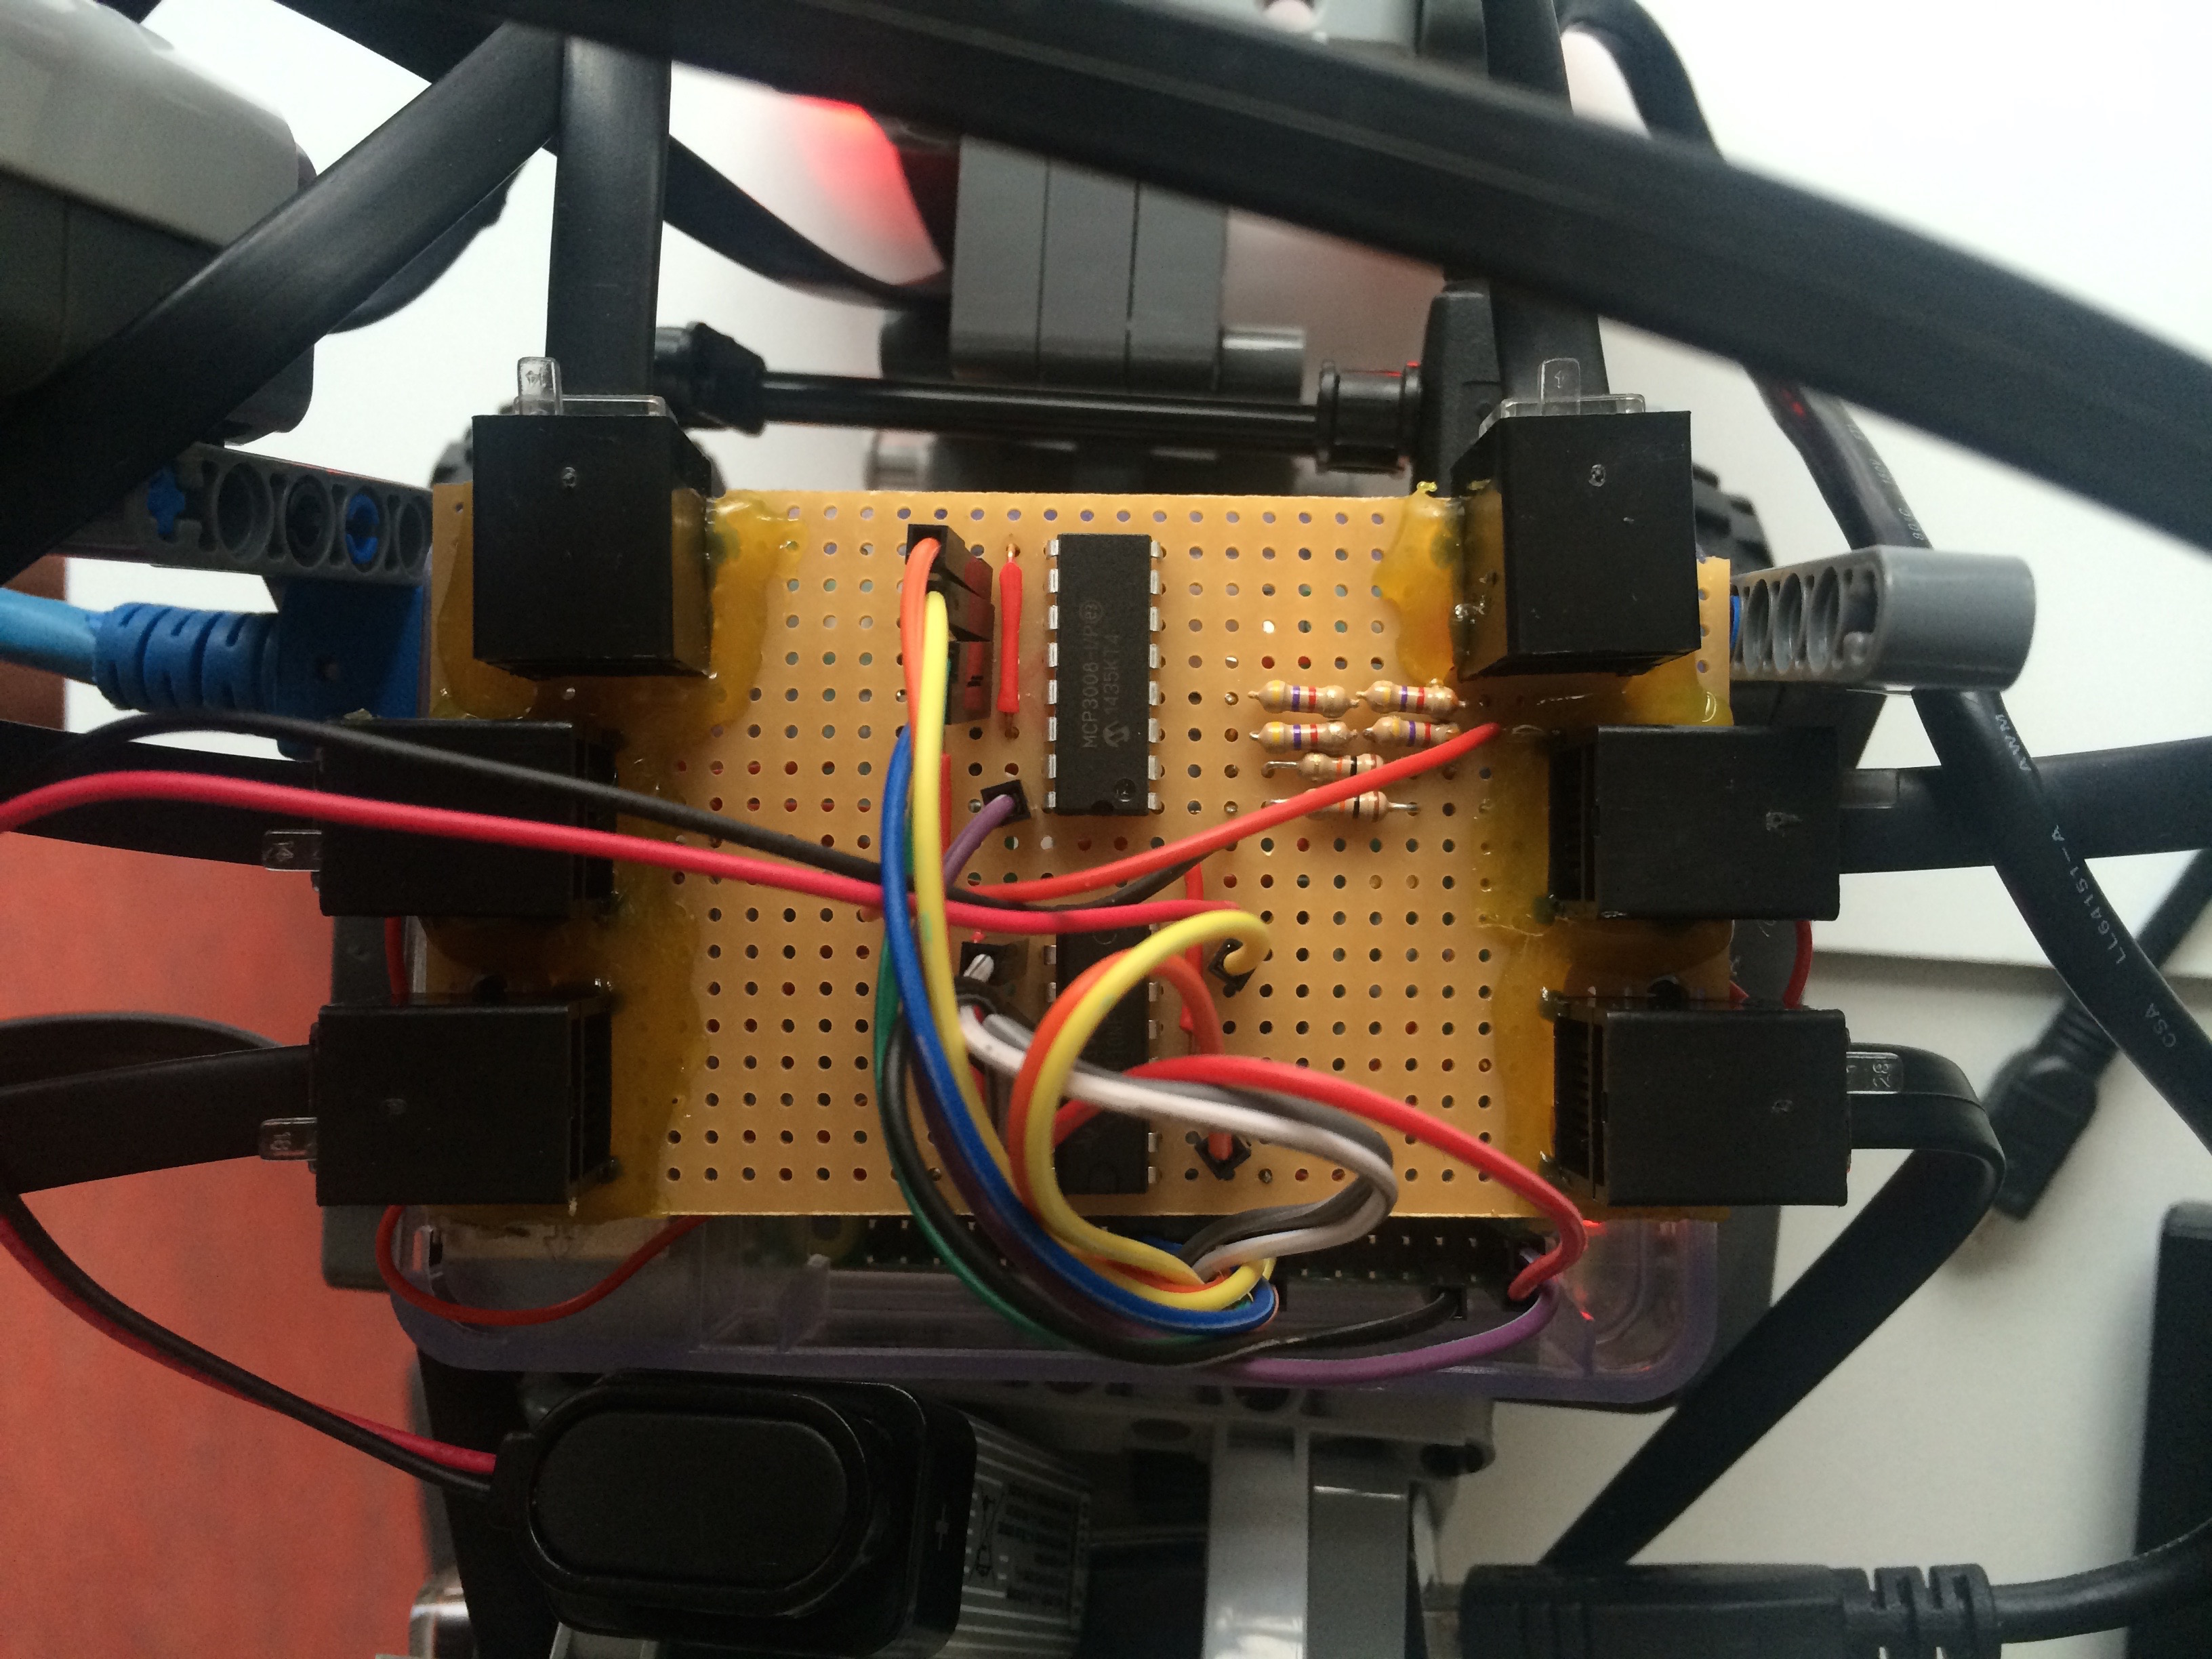
\includegraphics[width=12cm]{schaltung/komplett}
  \caption{Komplette Schaltung}
  \label{schaltung:komplett}
\end{figure}

\clearpage

\section{Herausforderungen beim Auslesen der Sensoren}

Den ersten Sensor den wir ausgelesen haben, war der Tastsensor. Diesen haben wir über einen GPIO direkt mit dem Raspberry PI verbunden.
Über das Öffnen des GPIOs via RPi.GPIO konnten wir auslesen, ob der Tastsensor gedrückt ist oder nicht. RPi.GPIO ist eine Bibliothek für Python, mit welcher die Kommunikation über GPIOs möglich ist.

Die Idee war den Lichtsensor auch über GPIO auslesen zu können. Eine solche Testkonfiguration zeigte allerdings, dass wir keine sinnvollen Werte über den GPIO auslesen können. 

Eine weitere Möglichkeit sahen wir darin, über I2C den Sensor auszulesen. Leider zeigte auch diese Option keinen Erfolg, da die NXT Sensoren ein eigenes I2C  Protokoll verwenden, welches nicht kompatibel ist mit dem I2C Bus am Raspberry PI. 

Eine funktionierende Lösung sah so aus, den Sensor mit einem A/D-Wandler zu verbinden und dann per GPIO die digital abgetasteten Daten zu empfangen. Da wir keinen A/D-Wandler zur Verfügung hatten, bauten wir uns einen eigenen A/D-Wandler. (vgl. Abbildung xx FIXME). Der Nachteil dieser Schaltung ist, dass lediglich ein Sensor ausgelessen werden kann. Um den Anforderungen gerecht zu werden und einen Parqour wie in der Robotik Vorlesung zu durchlaufen, ist der Einsatz von mehreren Sensoren notwendig. Dies erreichten wir mit dem Einsatz eines MCP3008 A/D-Wandler. Mit diesem ist das Auslesen von bis zu 8 Sensoren gleichzeitig möglich. (vergleiche xx FIXME). Wir haben es in dieser Arbeit nicht geschafft den Ultraschallsensor an den LegoPI anzubinden. Da dieser der einzige digitale Sensor von Lego Mindstorms ist, wird ein durchlafuen eines einfachen Parqours dennoch möglich sein.

\begin{figure}[h]
  \centering
  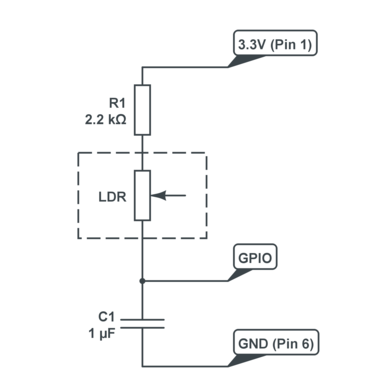
\includegraphics[width=10cm]{adwandlereigen}
  \caption{A/D-Wandler realisiert über einen LDR der in Reihe geschaltet ist mit einem 2.2 kOhm Widerstand und 1$\mu$F Kondensator}
  \label{Kap1:Lightsensor}
\end{figure}

\chapter{LegoPi-Software}
\label{Kap3}

Für die einfache Benutzung des LegoPi-Roboters wurde eine individuelle API entwickelt. Um den Wechsel zwischen der LeJOS Bibliothek, welche direkt auf den Lego Mindstorm-Komponenten ausgeführt wird, und der für den RaspberryPi entwickelten API so einfach wie möglich zu gestalten, ist diese stark an die LeJOS Software-Architektur angelehnt. Entwickelt wurde die API in der Programmiersprache Python und mithilfe der Bibliotheken RPi.GPIO, welche eine einfache Verwendung der RaspberryPi GPIO-Pins ermöglicht, sowie SpiDev um den SPI-Bus ansprechen zu können. Mithilfe der entwickelten API ist es möglich bis zu zwei Motoren und acht Sensoren zu steuern.

\section{Software-Komponenten}

Die LegoPi Software besteht aus vier grundlegenden Komponenten die einen einfachen Einstieg in die Benutzung gewährleisten.

\subsection{LegoPi.py - API}

In dem Python-Modul LegoPi sind alle in \autoref{Klassendiagramm} gezeigten Funktionalitäten eingebaut. Dieses Modul kann vom Entwickler genutzt werden um den individuellen Code für die Steuerung des LegoPi-Roboters zu kreieren.  

\subsection{Run.py - Individueller Code des Entwicklers}

Die \emph{Run.py}-Datei enthält den individuellen Code des entwicklers. Grund für die Vorgabe eines Dateinamens ist der in \autoref{subsec:execdaemon} beschriebene ExecDaemon.

\subsection{ExecDaemon.py - Automatischer Start des Entwickler-Codes}
\label{subsec:execdaemon}

Der ExecDaemon wird beim Starten des Systems automatisch ausgeführt. Er läuft im Hintergrund und wartet auf ein Signal des an \emph{Channel 3} angeschlossenen Tastsensors. Sobald dieses Signal empfangen wird, startet der ExecDaemon den in \emph{Run.py} eingetragenen Code. Dies ermöglicht es dem Entwickler den RaspberryPi vom Netzwerk zu trennen und den Code einfach zu testen, ohne ihn, zum Beispiel, direkt über eine SSH-Verbindung ausführen zu müssen.

\subsection{startup.sh - Vorbereitung des Systems}

Um das System unmittelbar nach Systemstart nutzen zu können, wird automatisch das Bash-Script \emph{startup.sh} ausgeführt. Dieses wird beim Neustart des Systems, durch einen in Crontab konfigurierten Job, automatisch ausgeführt. Dieses Script stellt zum einen sicher, dass der SPI-Bus aktiviert ist und zum anderen, dass der ExecDaemon ausgeführt wird.

\section{API}

Die API ist sehr einfach gestaltet und besteht aus wenigen Klassen, um die verschiedenen Sensoren und Motoren ansprechen zu können. 

\bild{Klassendiagramm}{17cm}{API - Klassendiagramm}

\clearpage % Alle Bilder, die bisher kamen ausgeben

\subsection{Motoren}
Die Motoren werden mithilfe eines übergebenen MotorPorts instanziiert. Dieser MotorPort beschreibt, an welchen GPIO Pins der Motor angeschlossen ist. Durch \emph{forward()} und \emph{backward()} lassen sich die Motoren vorwärts und rückwärts bewegen. Ebenfalls ist es möglich die Geschwindigkeit individuell anzupassen. Durch \emph{setSpeed(speed: int)} lässt sich eine Geschwindigkeit zwischen 0 und 100 angeben. 

\subsection{Sensoren}
Sensoren hingegen gibt es in zwei unterschiedlichen Spezialisierungen, dem Tastsensor (TouchSensor), sowie dem Lichtsensor (LightSensor). Beide sind eine Erweiterung der Klasse Sensor, welche Grundlegende Aufgaben übernimmt die für alle Sensor-Arten benötigt werden. Der Lichtsensor liefert mit seiner einzigen öffentlichen Methode \emph{getValue()} einen numerischen Wert zurück, der die Lichtreflektion beschreibt. Je geringer die Reflektion, desto kleiner ist auch der Rückgabewert. Zu beachten ist hier, dass durch unterschiedliche Lichtverhältnisse bedingt, verschiedene Werte zurückgeliefert werden können. Deshalb ist zu empfehlen, nicht nach einem konkreten Wert zu suchen, sondern ein gewisses Delta zuzulassen. Der Tastsensor bestitzt ebenfalls lediglich eine öffentliche Methode \emph{isPressed()}, welche einen booleschen Wert zurückliefert, ob der Tastsensor aktiviert wurde oder nicht. Sensoren werden mit einem übergebenen \emph{Channel} instanziiert. Dieser ist äquivalent zu den Channels am AD-Wandler, und beschreibt wo der Sensor angeschlossen ist. Da bist zu acht Sensoren genutzt werden können, wird eine Zahl zwischen null und sieben erwartet.

\subsection{Beispielanwendung}

Nachfolgend eine einfache Beispielanwendung, um das Verständnis der Programmierschnittstelle zu fördern.

\lstinputlisting[firstline=2,language=Python]{\srcloc/Run.py}

\chapter{Fazit}

In dieser Arbeit haben wir es geschafft LegoPI zu bauen. Einen Roboter der mit allen analogen Sensoren des Lego Mindstorms Bausatzes kompatibel ist. LegoPI ist ebenso in der Lage zwei Motoren zu steuern, um die Fortbewegung des Roboters zu ermöglichen. Wir konnten einen einfachen Parqour durchlaufen, in welchem der Roboter einer schwarzen Linie folgt und am Ende an einer Wand stehen bleibt. Das Signal zum Stehenbleiben wird hier über einen Tastsensor ausgelöst, welcher an der vorderen Front des Roboters angebracht ist.
